\documentclass[twoside]{book}

% Packages required by doxygen
\usepackage{fixltx2e}
\usepackage{calc}
\usepackage{doxygen}
\usepackage[export]{adjustbox} % also loads graphicx
\usepackage{graphicx}
\usepackage[utf8]{inputenc}
\usepackage{makeidx}
\usepackage{multicol}
\usepackage{multirow}
\PassOptionsToPackage{warn}{textcomp}
\usepackage{textcomp}
\usepackage[nointegrals]{wasysym}
\usepackage[table]{xcolor}

% Font selection
\usepackage[T1]{fontenc}
\usepackage[scaled=.90]{helvet}
\usepackage{courier}
\usepackage{amssymb}
\usepackage{sectsty}
\renewcommand{\familydefault}{\sfdefault}
\allsectionsfont{%
  \fontseries{bc}\selectfont%
  \color{darkgray}%
}
\renewcommand{\DoxyLabelFont}{%
  \fontseries{bc}\selectfont%
  \color{darkgray}%
}
\newcommand{\+}{\discretionary{\mbox{\scriptsize$\hookleftarrow$}}{}{}}

% Page & text layout
\usepackage{geometry}
\geometry{%
  a4paper,%
  top=2.5cm,%
  bottom=2.5cm,%
  left=2.5cm,%
  right=2.5cm%
}
\tolerance=750
\hfuzz=15pt
\hbadness=750
\setlength{\emergencystretch}{15pt}
\setlength{\parindent}{0cm}
\setlength{\parskip}{3ex plus 2ex minus 2ex}
\makeatletter
\renewcommand{\paragraph}{%
  \@startsection{paragraph}{4}{0ex}{-1.0ex}{1.0ex}{%
    \normalfont\normalsize\bfseries\SS@parafont%
  }%
}
\renewcommand{\subparagraph}{%
  \@startsection{subparagraph}{5}{0ex}{-1.0ex}{1.0ex}{%
    \normalfont\normalsize\bfseries\SS@subparafont%
  }%
}
\makeatother

% Headers & footers
\usepackage{fancyhdr}
\pagestyle{fancyplain}
\fancyhead[LE]{\fancyplain{}{\bfseries\thepage}}
\fancyhead[CE]{\fancyplain{}{}}
\fancyhead[RE]{\fancyplain{}{\bfseries\leftmark}}
\fancyhead[LO]{\fancyplain{}{\bfseries\rightmark}}
\fancyhead[CO]{\fancyplain{}{}}
\fancyhead[RO]{\fancyplain{}{\bfseries\thepage}}
\fancyfoot[LE]{\fancyplain{}{}}
\fancyfoot[CE]{\fancyplain{}{}}
\fancyfoot[RE]{\fancyplain{}{\bfseries\scriptsize Generated by Doxygen }}
\fancyfoot[LO]{\fancyplain{}{\bfseries\scriptsize Generated by Doxygen }}
\fancyfoot[CO]{\fancyplain{}{}}
\fancyfoot[RO]{\fancyplain{}{}}
\renewcommand{\footrulewidth}{0.4pt}
\renewcommand{\chaptermark}[1]{%
  \markboth{#1}{}%
}
\renewcommand{\sectionmark}[1]{%
  \markright{\thesection\ #1}%
}

% Indices & bibliography
\usepackage{natbib}
\usepackage[titles]{tocloft}
\setcounter{tocdepth}{3}
\setcounter{secnumdepth}{5}
\makeindex

% Hyperlinks (required, but should be loaded last)
\usepackage{ifpdf}
\ifpdf
  \usepackage[pdftex,pagebackref=true]{hyperref}
\else
  \usepackage[ps2pdf,pagebackref=true]{hyperref}
\fi
\hypersetup{%
  colorlinks=true,%
  linkcolor=blue,%
  citecolor=blue,%
  unicode%
}

% Custom commands
\newcommand{\clearemptydoublepage}{%
  \newpage{\pagestyle{empty}\cleardoublepage}%
}

\usepackage{caption}
\captionsetup{labelsep=space,justification=centering,font={bf},singlelinecheck=off,skip=4pt,position=top}

%===== C O N T E N T S =====

\begin{document}

% Titlepage & ToC
\hypersetup{pageanchor=false,
             bookmarksnumbered=true,
             pdfencoding=unicode
            }
\pagenumbering{roman}
\begin{titlepage}
\vspace*{7cm}
\begin{center}%
{\Large J\+A\+S\+PL \\[1ex]\large 0.\+1 }\\
\vspace*{1cm}
{\large Generated by Doxygen 1.8.11}\\
\end{center}
\end{titlepage}
\clearemptydoublepage
\tableofcontents
\clearemptydoublepage
\pagenumbering{arabic}
\hypersetup{pageanchor=true}

%--- Begin generated contents ---
\chapter{Class Index}
\section{Class List}
Here are the classes, structs, unions and interfaces with brief descriptions\+:\begin{DoxyCompactList}
\item\contentsline{section}{\hyperlink{classjaspl_1_1ocl_1_1_f_f_t}{jaspl\+::ocl\+::\+F\+F\+T$<$ T $>$} }{\pageref{classjaspl_1_1ocl_1_1_f_f_t}}{}
\item\contentsline{section}{\hyperlink{classjaspl_1_1has__accessor}{jaspl\+::has\+\_\+accessor$<$ T $>$} }{\pageref{classjaspl_1_1has__accessor}}{}
\item\contentsline{section}{\hyperlink{structjaspl_1_1has__begin__end}{jaspl\+::has\+\_\+begin\+\_\+end$<$ T $>$} }{\pageref{structjaspl_1_1has__begin__end}}{}
\item\contentsline{section}{\hyperlink{structjaspl_1_1has__const__iterator}{jaspl\+::has\+\_\+const\+\_\+iterator$<$ T $>$} }{\pageref{structjaspl_1_1has__const__iterator}}{}
\item\contentsline{section}{\hyperlink{classjaspl_1_1has__data}{jaspl\+::has\+\_\+data$<$ T $>$} }{\pageref{classjaspl_1_1has__data}}{}
\item\contentsline{section}{\hyperlink{classjaspl_1_1has__data2}{jaspl\+::has\+\_\+data2$<$ T, Args $>$} }{\pageref{classjaspl_1_1has__data2}}{}
\item\contentsline{section}{\hyperlink{classjaspl_1_1has__size}{jaspl\+::has\+\_\+size$<$ T $>$} }{\pageref{classjaspl_1_1has__size}}{}
\item\contentsline{section}{\hyperlink{structjaspl_1_1is__stdlib__container}{jaspl\+::is\+\_\+stdlib\+\_\+container$<$ T $>$} }{\pageref{structjaspl_1_1is__stdlib__container}}{}
\item\contentsline{section}{\hyperlink{class_j_chart}{J\+Chart} }{\pageref{class_j_chart}}{}
\item\contentsline{section}{\hyperlink{classjaspl_1_1_j_f_f_t}{jaspl\+::\+J\+F\+F\+T$<$ T $>$} }{\pageref{classjaspl_1_1_j_f_f_t}}{}
\item\contentsline{section}{\hyperlink{classjaspl_1_1_j_filter}{jaspl\+::\+J\+Filter} }{\pageref{classjaspl_1_1_j_filter}}{}
\item\contentsline{section}{\hyperlink{classjaspl_1_1j_filter_unit_test}{jaspl\+::j\+Filter\+Unit\+Test$<$ T $>$} }{\pageref{classjaspl_1_1j_filter_unit_test}}{}
\item\contentsline{section}{\hyperlink{class_j_non_linear_filter}{J\+Non\+Linear\+Filter} }{\pageref{class_j_non_linear_filter}}{}
\item\contentsline{section}{\hyperlink{classjaspl_1_1_j_vector}{jaspl\+::\+J\+Vector$<$ F $>$} }{\pageref{classjaspl_1_1_j_vector}}{}
\item\contentsline{section}{\hyperlink{classjaspl_1_1ocl_1_1_linear_convolution}{jaspl\+::ocl\+::\+Linear\+Convolution$<$ T $>$} }{\pageref{classjaspl_1_1ocl_1_1_linear_convolution}}{}
\item\contentsline{section}{\hyperlink{classjaspl_1_1ocl_1_1_non_linear_convolution}{jaspl\+::ocl\+::\+Non\+Linear\+Convolution$<$ T $>$} }{\pageref{classjaspl_1_1ocl_1_1_non_linear_convolution}}{}
\item\contentsline{section}{\hyperlink{classjaspl_1_1ocl_1_1_open_c_l_base}{jaspl\+::ocl\+::\+Open\+C\+L\+Base} \\*Base class for every class that needs access to Open\+CL Platforms, Contexts or Devices }{\pageref{classjaspl_1_1ocl_1_1_open_c_l_base}}{}
\item\contentsline{section}{\hyperlink{classjaspl_1_1ouroborus}{jaspl\+::ouroborus$<$ T $>$} }{\pageref{classjaspl_1_1ouroborus}}{}
\item\contentsline{section}{\hyperlink{classjaspl_1_1_plotter}{jaspl\+::\+Plotter$<$ T $>$} }{\pageref{classjaspl_1_1_plotter}}{}
\item\contentsline{section}{\hyperlink{classjaspl_1_1ocl_1_1_power_spectrum}{jaspl\+::ocl\+::\+Power\+Spectrum$<$ T $>$} }{\pageref{classjaspl_1_1ocl_1_1_power_spectrum}}{}
\item\contentsline{section}{\hyperlink{classjaspl_1_1ocl_1_1_rebin}{jaspl\+::ocl\+::\+Rebin} }{\pageref{classjaspl_1_1ocl_1_1_rebin}}{}
\item\contentsline{section}{\hyperlink{classjaspl_1_1_recurse_mean}{jaspl\+::\+Recurse\+Mean$<$ T $>$} \\*Average together a (nearly) arbitrary number of container-\/like objects using the recursive definition of the expected value defined by\+: }{\pageref{classjaspl_1_1_recurse_mean}}{}
\item\contentsline{section}{\hyperlink{classjaspl_1_1ocl_1_1_scalar_add}{jaspl\+::ocl\+::\+Scalar\+Add$<$ T $>$} }{\pageref{classjaspl_1_1ocl_1_1_scalar_add}}{}
\item\contentsline{section}{\hyperlink{classjaspl_1_1ocl_1_1_scalar_multiply}{jaspl\+::ocl\+::\+Scalar\+Multiply$<$ T $>$} }{\pageref{classjaspl_1_1ocl_1_1_scalar_multiply}}{}
\item\contentsline{section}{\hyperlink{classjaspl_1_1ocl_1_1_task_item}{jaspl\+::ocl\+::\+Task\+Item} }{\pageref{classjaspl_1_1ocl_1_1_task_item}}{}
\item\contentsline{section}{\hyperlink{classjaspl_1_1ocl_1_1_task_queue}{jaspl\+::ocl\+::\+Task\+Queue$<$ T $>$} }{\pageref{classjaspl_1_1ocl_1_1_task_queue}}{}
\item\contentsline{section}{\hyperlink{classjaspl_1_1ocl_1_1_task_queue_3_01_t_01_5_01_4}{jaspl\+::ocl\+::\+Task\+Queue$<$ T $\ast$ $>$} }{\pageref{classjaspl_1_1ocl_1_1_task_queue_3_01_t_01_5_01_4}}{}
\item\contentsline{section}{\hyperlink{classjaspl_1_1ocl_1_1_task_queue_base}{jaspl\+::ocl\+::\+Task\+Queue\+Base} \\*The fundamental structure underlying all Open\+CL Functions }{\pageref{classjaspl_1_1ocl_1_1_task_queue_base}}{}
\end{DoxyCompactList}

\chapter{Class Documentation}
\hypertarget{classjaspl_1_1_j_f_f_t}{}\section{jaspl\+:\+:J\+F\+FT Class Reference}
\label{classjaspl_1_1_j_f_f_t}\index{jaspl\+::\+J\+F\+FT@{jaspl\+::\+J\+F\+FT}}
\subsection*{Public Member Functions}
\begin{DoxyCompactItemize}
\item 
void {\bfseries Setup} (uint size)\hypertarget{classjaspl_1_1_j_f_f_t_a9ae772905c4f41a2de1c8b62683f6b5e}{}\label{classjaspl_1_1_j_f_f_t_a9ae772905c4f41a2de1c8b62683f6b5e}

\item 
{\footnotesize template$<$typename T $>$ }\\void {\bfseries Power\+Spectrum} (T \&input)\hypertarget{classjaspl_1_1_j_f_f_t_a3953d73759cf17cb93f2b1e76691a8fe}{}\label{classjaspl_1_1_j_f_f_t_a3953d73759cf17cb93f2b1e76691a8fe}

\item 
void {\bfseries Tear\+Down} ()\hypertarget{classjaspl_1_1_j_f_f_t_a7ba090708a0e3b6e1dba81574fa52548}{}\label{classjaspl_1_1_j_f_f_t_a7ba090708a0e3b6e1dba81574fa52548}

\end{DoxyCompactItemize}


\subsection{Detailed Description}


Definition at line 15 of file jfft.\+h.


\hypertarget{classjaspl_1_1ocl_1_1_j_f_f_t}{}\section{jaspl\+:\+:ocl\+:\+:J\+F\+FT Class Reference}
\label{classjaspl_1_1ocl_1_1_j_f_f_t}\index{jaspl\+::ocl\+::\+J\+F\+FT@{jaspl\+::ocl\+::\+J\+F\+FT}}
\subsection*{Public Member Functions}
\begin{DoxyCompactItemize}
\item 
void {\bfseries List\+C\+L\+Devices} ()\hypertarget{classjaspl_1_1ocl_1_1_j_f_f_t_a345a5366d1bfc966d6e0b5932b2624d8}{}\label{classjaspl_1_1ocl_1_1_j_f_f_t_a345a5366d1bfc966d6e0b5932b2624d8}

\item 
void {\bfseries Setup} ()\hypertarget{classjaspl_1_1ocl_1_1_j_f_f_t_ad68656a8859214cea4bb4ed5dca93995}{}\label{classjaspl_1_1ocl_1_1_j_f_f_t_ad68656a8859214cea4bb4ed5dca93995}

\item 
{\footnotesize template$<$typename T $>$ }\\void {\bfseries Power\+Spectrum} (T \&input)\hypertarget{classjaspl_1_1ocl_1_1_j_f_f_t_a2d41202ab9b3231f1c347cd8cbc465f3}{}\label{classjaspl_1_1ocl_1_1_j_f_f_t_a2d41202ab9b3231f1c347cd8cbc465f3}

\item 
void {\bfseries Teardown} ()\hypertarget{classjaspl_1_1ocl_1_1_j_f_f_t_aca6fb3c6a7f7d7c7d04aeac51b2b8c2f}{}\label{classjaspl_1_1ocl_1_1_j_f_f_t_aca6fb3c6a7f7d7c7d04aeac51b2b8c2f}

\end{DoxyCompactItemize}


\subsection{Detailed Description}


Definition at line 21 of file ocl\+\_\+jfft.\+h.


\hypertarget{classjaspl_1_1_j_filter}{}\section{jaspl\+:\+:J\+Filter Class Reference}
\label{classjaspl_1_1_j_filter}\index{jaspl\+::\+J\+Filter@{jaspl\+::\+J\+Filter}}


\subsection{Detailed Description}


Definition at line 21 of file jlinearfilter.\+h.


\hypertarget{classjaspl_1_1ocl_1_1_j_linear_convolve}{}\section{jaspl\+:\+:ocl\+:\+:J\+Linear\+Convolve Class Reference}
\label{classjaspl_1_1ocl_1_1_j_linear_convolve}\index{jaspl\+::ocl\+::\+J\+Linear\+Convolve@{jaspl\+::ocl\+::\+J\+Linear\+Convolve}}


Inheritance diagram for jaspl\+:\+:ocl\+:\+:J\+Linear\+Convolve\+:
\nopagebreak
\begin{figure}[H]
\begin{center}
\leavevmode
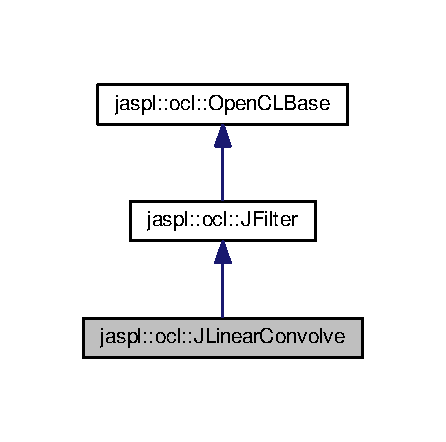
\includegraphics[width=214pt]{classjaspl_1_1ocl_1_1_j_linear_convolve__inherit__graph}
\end{center}
\end{figure}


Collaboration diagram for jaspl\+:\+:ocl\+:\+:J\+Linear\+Convolve\+:
\nopagebreak
\begin{figure}[H]
\begin{center}
\leavevmode
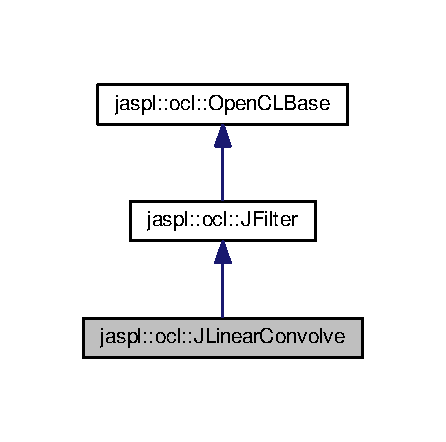
\includegraphics[width=214pt]{classjaspl_1_1ocl_1_1_j_linear_convolve__coll__graph}
\end{center}
\end{figure}
\subsection*{Public Member Functions}
\begin{DoxyCompactItemize}
\item 
{\bfseries J\+Linear\+Convolve} (uint device\+\_\+number=0)\hypertarget{classjaspl_1_1ocl_1_1_j_linear_convolve_ac23d0dd668a469eb7ea80197c0074479}{}\label{classjaspl_1_1ocl_1_1_j_linear_convolve_ac23d0dd668a469eb7ea80197c0074479}

\item 
{\footnotesize template$<$class T $>$ }\\\hyperlink{classjaspl_1_1_j_vector}{J\+Vector}$<$ T $>$ {\bfseries Convolve} (\hyperlink{classjaspl_1_1_j_vector}{J\+Vector}$<$ T $>$ \&signal, \hyperlink{classjaspl_1_1_j_vector}{J\+Vector}$<$ T $>$ \&kernel)\hypertarget{classjaspl_1_1ocl_1_1_j_linear_convolve_a49242f52e8286cdb0844d15b5339fb6a}{}\label{classjaspl_1_1ocl_1_1_j_linear_convolve_a49242f52e8286cdb0844d15b5339fb6a}

\end{DoxyCompactItemize}
\subsection*{Additional Inherited Members}


\subsection{Detailed Description}


Definition at line 27 of file ocl\+\_\+jlinearfilter.\+h.


\hypertarget{classjaspl_1_1_j_vector}{}\section{jaspl\+:\+:J\+Vector$<$ F $>$ Class Template Reference}
\label{classjaspl_1_1_j_vector}\index{jaspl\+::\+J\+Vector$<$ F $>$@{jaspl\+::\+J\+Vector$<$ F $>$}}
\subsection*{Public Member Functions}
\begin{DoxyCompactItemize}
\item 
{\bfseries J\+Vector} (std\+::string raw\+\_\+data)\hypertarget{classjaspl_1_1_j_vector_aec9bccd8f55bdb1977f02fccc7872d86}{}\label{classjaspl_1_1_j_vector_aec9bccd8f55bdb1977f02fccc7872d86}

\item 
{\bfseries J\+Vector} (std\+::vector$<$ F $>$ vec)\hypertarget{classjaspl_1_1_j_vector_ab9a8bee6860dc4ddd3c899b73de93e54}{}\label{classjaspl_1_1_j_vector_ab9a8bee6860dc4ddd3c899b73de93e54}

\item 
{\bfseries J\+Vector} (F $\ast$ptr, uint ptr\+\_\+size)\hypertarget{classjaspl_1_1_j_vector_ae3cee2406660cf6bdd73fd416ca23835}{}\label{classjaspl_1_1_j_vector_ae3cee2406660cf6bdd73fd416ca23835}

\item 
{\bfseries J\+Vector} (uint size)\hypertarget{classjaspl_1_1_j_vector_a91890a543ea9a946a56f616dd9748bcd}{}\label{classjaspl_1_1_j_vector_a91890a543ea9a946a56f616dd9748bcd}

\item 
{\bfseries J\+Vector} (uint size, F fill\+\_\+element)\hypertarget{classjaspl_1_1_j_vector_aea6660117c28bd9a787a3318f3e2c0ec}{}\label{classjaspl_1_1_j_vector_aea6660117c28bd9a787a3318f3e2c0ec}

\item 
\hyperlink{classjaspl_1_1_j_vector}{J\+Vector}$<$ F $>$ {\bfseries operator$\ast$=} (F scalar)\hypertarget{classjaspl_1_1_j_vector_a401ed55d69adaae0850b31082694313f}{}\label{classjaspl_1_1_j_vector_a401ed55d69adaae0850b31082694313f}

\item 
\hyperlink{classjaspl_1_1_j_vector}{J\+Vector}$<$ F $>$ {\bfseries operator$\ast$} (F scalar)\hypertarget{classjaspl_1_1_j_vector_a6e882f97e2c212aebe83817924633099}{}\label{classjaspl_1_1_j_vector_a6e882f97e2c212aebe83817924633099}

\item 
\hyperlink{classjaspl_1_1_j_vector}{J\+Vector}$<$ F $>$ {\bfseries operator+=} (F scalar)\hypertarget{classjaspl_1_1_j_vector_a159125c3544f643484a088391af523c4}{}\label{classjaspl_1_1_j_vector_a159125c3544f643484a088391af523c4}

\item 
void {\bfseries push\+\_\+back} (F element)\hypertarget{classjaspl_1_1_j_vector_a8906043d61595e7737c59706c9ac7643}{}\label{classjaspl_1_1_j_vector_a8906043d61595e7737c59706c9ac7643}

\item 
void {\bfseries push\+\_\+front} (F element)\hypertarget{classjaspl_1_1_j_vector_ada7d072df43b19a445f00fc7e9a36e25}{}\label{classjaspl_1_1_j_vector_ada7d072df43b19a445f00fc7e9a36e25}

\item 
std\+::vector$<$ F $>$\+::iterator {\bfseries begin} ()\hypertarget{classjaspl_1_1_j_vector_ade0638fb564d0c859abdbdc23ba97fa3}{}\label{classjaspl_1_1_j_vector_ade0638fb564d0c859abdbdc23ba97fa3}

\item 
std\+::vector$<$ F $>$\+::iterator {\bfseries end} ()\hypertarget{classjaspl_1_1_j_vector_a47d157a58ee97a0b7170f1cff4f70511}{}\label{classjaspl_1_1_j_vector_a47d157a58ee97a0b7170f1cff4f70511}

\item 
F $\ast$ {\bfseries data} ()\hypertarget{classjaspl_1_1_j_vector_ad52b5a350b0e408a9158cc4c6eba7d0f}{}\label{classjaspl_1_1_j_vector_ad52b5a350b0e408a9158cc4c6eba7d0f}

\item 
F \& {\bfseries operator\mbox{[}$\,$\mbox{]}} (const uint index)\hypertarget{classjaspl_1_1_j_vector_a077310d6ba37aa477e70bfceaa79e916}{}\label{classjaspl_1_1_j_vector_a077310d6ba37aa477e70bfceaa79e916}

\item 
F \& {\bfseries at} (const uint index)\hypertarget{classjaspl_1_1_j_vector_a199548bafdcf1f257368a27ec6243069}{}\label{classjaspl_1_1_j_vector_a199548bafdcf1f257368a27ec6243069}

\item 
void {\bfseries reserve} (uint n)\hypertarget{classjaspl_1_1_j_vector_a4d1ff6d9b08324a8db47087dc5c64efc}{}\label{classjaspl_1_1_j_vector_a4d1ff6d9b08324a8db47087dc5c64efc}

\item 
double {\bfseries norm} ()\hypertarget{classjaspl_1_1_j_vector_a7811d30c896a5411fb8e23d290437f92}{}\label{classjaspl_1_1_j_vector_a7811d30c896a5411fb8e23d290437f92}

\item 
void {\bfseries Normalize} ()\hypertarget{classjaspl_1_1_j_vector_a2144d5df7ed2c44ccd6e43aa586ec484}{}\label{classjaspl_1_1_j_vector_a2144d5df7ed2c44ccd6e43aa586ec484}

\item 
double {\bfseries std\+\_\+dev} ()\hypertarget{classjaspl_1_1_j_vector_a26ad1598c827f28aeb159f036a890c1c}{}\label{classjaspl_1_1_j_vector_a26ad1598c827f28aeb159f036a890c1c}

\item 
double {\bfseries mean} ()\hypertarget{classjaspl_1_1_j_vector_a14a30029d1e440c09f8353b0eb9f8fa0}{}\label{classjaspl_1_1_j_vector_a14a30029d1e440c09f8353b0eb9f8fa0}

\item 
F {\bfseries min} ()\hypertarget{classjaspl_1_1_j_vector_a6bb1cfc7f6c73526cc079a20994abfcd}{}\label{classjaspl_1_1_j_vector_a6bb1cfc7f6c73526cc079a20994abfcd}

\item 
F {\bfseries max} ()\hypertarget{classjaspl_1_1_j_vector_a670b6ae1e2becf0f0c311483ff7ae8b1}{}\label{classjaspl_1_1_j_vector_a670b6ae1e2becf0f0c311483ff7ae8b1}

\item 
uint {\bfseries size} ()\hypertarget{classjaspl_1_1_j_vector_a704189ad3e7f18bc6c2a42df23ce20eb}{}\label{classjaspl_1_1_j_vector_a704189ad3e7f18bc6c2a42df23ce20eb}

\end{DoxyCompactItemize}
\subsection*{Friends}
\begin{DoxyCompactItemize}
\item 
{\footnotesize template$<$class T $>$ }\\void {\bfseries plot} (\hyperlink{classjaspl_1_1_j_vector}{J\+Vector}$<$ T $>$ \&vec)\hypertarget{classjaspl_1_1_j_vector_a6dc51c5dfdd4aacdf08ebad6d0d2afae}{}\label{classjaspl_1_1_j_vector_a6dc51c5dfdd4aacdf08ebad6d0d2afae}

\item 
{\footnotesize template$<$class T $>$ }\\void {\bfseries plot} (\hyperlink{classjaspl_1_1_j_vector}{J\+Vector}$<$ T $>$ \&vec, std\+::string plot\+\_\+title)\hypertarget{classjaspl_1_1_j_vector_a61b154a38160f96e7326fa73252f59ff}{}\label{classjaspl_1_1_j_vector_a61b154a38160f96e7326fa73252f59ff}

\item 
bool {\bfseries operator==} (\hyperlink{classjaspl_1_1_j_vector}{J\+Vector}$<$ F $>$ \&vector\+\_\+a, \hyperlink{classjaspl_1_1_j_vector}{J\+Vector}$<$ F $>$ \&vector\+\_\+b)\hypertarget{classjaspl_1_1_j_vector_a81fad03b34e80d689ede7e6d7178ed56}{}\label{classjaspl_1_1_j_vector_a81fad03b34e80d689ede7e6d7178ed56}

\item 
bool {\bfseries operator!=} (\hyperlink{classjaspl_1_1_j_vector}{J\+Vector}$<$ F $>$ \&vector\+\_\+a, \hyperlink{classjaspl_1_1_j_vector}{J\+Vector}$<$ F $>$ \&vector\+\_\+b)\hypertarget{classjaspl_1_1_j_vector_ad9f0b4638213ca7ffad3c23031a58c35}{}\label{classjaspl_1_1_j_vector_ad9f0b4638213ca7ffad3c23031a58c35}

\item 
std\+::ostream \& {\bfseries operator$<$$<$} (std\+::ostream \&stream, \hyperlink{classjaspl_1_1_j_vector}{J\+Vector}$<$ F $>$ \&spectrum)\hypertarget{classjaspl_1_1_j_vector_a5bb4330c3ad441ee4a22dd90c019f20d}{}\label{classjaspl_1_1_j_vector_a5bb4330c3ad441ee4a22dd90c019f20d}

\item 
std\+::ofstream \& {\bfseries operator$<$$<$} (std\+::ofstream \&stream, \hyperlink{classjaspl_1_1_j_vector}{J\+Vector}$<$ F $>$ \&spectrum)\hypertarget{classjaspl_1_1_j_vector_aa520fbd88b8c88fc26f1d352ac911f37}{}\label{classjaspl_1_1_j_vector_aa520fbd88b8c88fc26f1d352ac911f37}

\item 
\hyperlink{classjaspl_1_1_j_vector}{J\+Vector}$<$ F $>$ {\bfseries operator+} (\hyperlink{classjaspl_1_1_j_vector}{J\+Vector}$<$ F $>$ \&vector\+\_\+a, \hyperlink{classjaspl_1_1_j_vector}{J\+Vector}$<$ F $>$ \&vector\+\_\+b)\hypertarget{classjaspl_1_1_j_vector_ab0c3db97c64f145b82254682de3a9dac}{}\label{classjaspl_1_1_j_vector_ab0c3db97c64f145b82254682de3a9dac}

\item 
\hyperlink{classjaspl_1_1_j_vector}{J\+Vector}$<$ F $>$ {\bfseries operator+} (\hyperlink{classjaspl_1_1_j_vector}{J\+Vector}$<$ F $>$ \&vector\+\_\+a, std\+::vector$<$ F $>$ \&vector\+\_\+b)\hypertarget{classjaspl_1_1_j_vector_a2d32b7256486f2427723aa03d2e21016}{}\label{classjaspl_1_1_j_vector_a2d32b7256486f2427723aa03d2e21016}

\item 
\hyperlink{classjaspl_1_1_j_vector}{J\+Vector}$<$ F $>$ {\bfseries operator-\/} (\hyperlink{classjaspl_1_1_j_vector}{J\+Vector}$<$ F $>$ \&vector\+\_\+a, \hyperlink{classjaspl_1_1_j_vector}{J\+Vector}$<$ F $>$ \&vector\+\_\+b)\hypertarget{classjaspl_1_1_j_vector_a0346f9409f8dbf1c202a587bd4be6e6d}{}\label{classjaspl_1_1_j_vector_a0346f9409f8dbf1c202a587bd4be6e6d}

\item 
\hyperlink{classjaspl_1_1_j_vector}{J\+Vector}$<$ F $>$ {\bfseries operator-\/} (\hyperlink{classjaspl_1_1_j_vector}{J\+Vector}$<$ F $>$ \&vector\+\_\+a, std\+::vector$<$ F $>$ \&vector\+\_\+b)\hypertarget{classjaspl_1_1_j_vector_ae6badaa441ef27ab6140d8dcec31eae8}{}\label{classjaspl_1_1_j_vector_ae6badaa441ef27ab6140d8dcec31eae8}

\item 
\hyperlink{classjaspl_1_1_j_vector}{J\+Vector}$<$ F $>$ {\bfseries operator$\ast$} (\hyperlink{classjaspl_1_1_j_vector}{J\+Vector}$<$ F $>$ \&vector\+\_\+a, \hyperlink{classjaspl_1_1_j_vector}{J\+Vector}$<$ F $>$ \&vector\+\_\+b)\hypertarget{classjaspl_1_1_j_vector_a2c5ea5529b0e58fd7cca8431b618d909}{}\label{classjaspl_1_1_j_vector_a2c5ea5529b0e58fd7cca8431b618d909}

\item 
\hyperlink{classjaspl_1_1_j_vector}{J\+Vector}$<$ F $>$ {\bfseries operator$\ast$} (\hyperlink{classjaspl_1_1_j_vector}{J\+Vector}$<$ F $>$ \&vector\+\_\+a, std\+::vector$<$ F $>$ \&vector\+\_\+b)\hypertarget{classjaspl_1_1_j_vector_a357e9f8d65a0e055329173fc96a269dc}{}\label{classjaspl_1_1_j_vector_a357e9f8d65a0e055329173fc96a269dc}

\end{DoxyCompactItemize}


\subsection{Detailed Description}
\subsubsection*{template$<$class F$>$\\*
class jaspl\+::\+J\+Vector$<$ F $>$}



Definition at line 20 of file jvector.\+h.


%--- End generated contents ---

% Index
\backmatter
\newpage
\phantomsection
\clearemptydoublepage
\addcontentsline{toc}{chapter}{Index}
\printindex

\end{document}
